\section{Work, Energy and Power}
%\begin{center}
%$\text{\textbf{Work}} = \text{Force} \times \text{distance in direction of Force} $\\
%Unit = 1 N $\times$ m = 1 J (Joule)\\
%\textbf{Energy} is the ability to do work. Unit = 1 J (Joule)\\
%$\text{\textbf{Power}} = \text{Work Done} \div \text{time} $\\
%Unit = 1 J $\div$ 1 s = 1 W (Watt)
%\end{center}

\begin{multicols}{2}


\section*{Work}


\subsection{Work Done by Lifting}

\begin{center}
\includegraphics[width=0.25\textwidth]{./img/source/work-lifting.png}
\end{center}

\begin{description*}
%\item[Subtopic:]{}
\item[Materials:]{\nameref{sec:spring-balance}, block of wood, ruler}
%\item[Setup:]{}
\item[Procedure:]{Raise a block of wood from a table using a spring balance. Read the balance while lifting at \emph{constant velocity}, not when starting or stopping. Compare this to the weight of the block. Measure the vertical distance raised $h$. }
%\item[Hazards:]{}
%\item[Questions:]{Calculate the work done when the block is raised a vertical distance $h$.}
%\item[Observations:]{}
\item[Theory:]{$\text{Work done} = \text{Weight} \times h$}
%\item[Applications:]{}
%\item[Notes:]{}
\end{description*}

\subsection{Work Done by Friction}

\begin{center}
\includegraphics[width=0.4\textwidth]{./img/source/work-friction.png}
\end{center}

\begin{description*}
%\item[Subtopic:]{}
\item[Materials:]{\nameref{sec:spring-balance}, block of wood, ruler}
%\item[Setup:]{}
\item[Procedure:]{Place the block of wood on a table and pull with constant velocity using a spring balance. Measure the distance moved by the block.}
%\item[Hazards:]{}
%\item[Questions:]{Calculate the work done from the spring balance and measured distance $x$.}
%\item[Observations:]{}
\item[Theory:]{Because the block is moving at constant velocity (no net force), the force which pulls the block is equal to the force of friction and opposite in magnitude. Thus, $\text{Work done} = \text{Force of friction} \times x$}
%\item[Applications:]{}
%\item[Notes:]{}
\end{description*}

%==================================================================================================%

\section*{Energy}


\subsection{Forms of Energy}

\begin{center}
\includegraphics[width=0.5\textwidth]{./img/vso/forms-energy.jpg}
\end{center}

\begin{description*}
%\item[Subtopic:]{}
%\item[Materials:]{}
%\item[Setup:]{}
%\item[Procedure:]{}
%\item[Hazards:]{}
%\item[Questions:]{}
%\item[Observations:]{}
\item[Theory:]{Energy can take many forms, including potential, kinetic, chemical, heat, sound and electrical. \emph{Potential energy} is energy which is stored is some medium, e.g. spring or battery. \emph{Kinetic energy} is energy in motion, e.g. football or running person.}
\item[Applications:]{What other examples of energy can be found in our daily lives?}
%\item[Notes:]{}
\end{description*}

\subsection{A Slingshot}

\begin{center}
\includegraphics[width=0.4\textwidth]{./img/source/slingshot.png}
\end{center}

\begin{description*}
%\item[Subtopic:]{}
\item[Materials:]{Rubber band, branched stick, stone}
%\item[Setup:]{}
\item[Procedure:]{Tie either end of a rubber band to the branches of the stick. Place a stone in the middle of the band, pull back and release.}
\item[Hazards:]{Aim the slingshot away from all people.}
%\item[Questions:]{}
%\item[Observations:]{}
\item[Theory:]{The rubber band stores potential energy when stretched, which is transferred to the stone as kinetic energy upon release.}
%\item[Applications:]{}
\item[Notes:]{Conduct an experiment to determine the relationship between stretched length of the rubber band and distance traveled by the stone.}
\end{description*}

\subsection[Potential Energy of a Clothespin]{Potential Energy of a \hfill \\ Clothespin}

\begin{center}
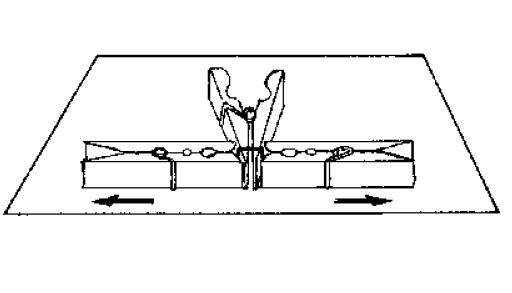
\includegraphics[width=0.45\textwidth]{./img/source/energy-clothespin.png}
\end{center}

\begin{description*}
%\item[Subtopic:]{}
\item[Materials:]{Three clothespins, scissors}
%\item[Setup:]{}
\item[Procedure:]{Tie the handles of a spring clothespin together with one loop of string. Place it in between two other clothespins on a flat table as shown. Cut or burn the string.}
%\item[Hazards:]{}
%\item[Questions:]{}
\item[Observations:]{The two clothespins on either side fly off in opposite directions.}
\item[Theory:]{The spring in the clothespin stores potential energy which is released when the string is cut. This energy is converted into kinetic energy, seen by the movement of the other clothespins.}
%\item[Applications:]{}
%\item[Notes:]{}
\end{description*}

\subsection{The Steam Engine}

\begin{center}
\includegraphics[width=0.49\textwidth]{./img/vso/steam-engine.jpg}
\end{center}

\begin{description*}
%\item[Subtopic:]{}
\item[Materials:]{Tin can with lid, pin, cork, \nameref{sec:heatsources}, 2 straws}
\item[Setup:]{Poke a small hole near the top of the tin can. Make sure the lid fits tightly, but has a safety bung (i.e. cork). Mount a straw on a pin so that it may spin freely.}
\item[Procedure:]{Fill the can half way with water and heat until boiling. Hold the straw spinner near the hole in the tin.}
\item[Hazards:]{Make sure the safety bung is not too tight and that the tin is not filled with water.}
%\item[Questions:]{}
%\item[Observations:]{}
\item[Theory:]{The candle or burner transfers heat energy to the tin and hence water. This heat energy in the water molecules is converted to kinetic energy as they are forced out of the tin hole. This mechanical energy is transferred to the spinner and makes it turn.}
\item[Applications:]{Mount the steam engine to a small raft and place in water to make a steam boat.}
%\item[Notes:]{}
\end{description*}

\columnbreak

\subsection{The Simple Pendulum}

\begin{center}
\includegraphics[width=0.2\textwidth]{./img/source/pendulum.png}
\end{center}

\begin{description*}
%\item[Subtopic:]{}
\item[Materials:]{Stone, string}
%\item[Setup:]{}
\item[Procedure:]{Suspend a stone on a long string and hang from a table. Displace the pendulum to one side and release.}
%\item[Hazards:]{}
%\item[Questions:]{}
\item[Observations:]{The pendulum swings back and forth at near regular intervals.}
\item[Theory:]{When the pendulum is released from one side, it has a maximum height and hence potential energy (P.E.), but no kinetic energy (K.E.). When it reaches the low point of its swing, it has maximum velocity and hence K.E., but its P.E. is a minimum. Thus the pendulum's energy is constantly being converted between P.E. and K.E.}
%\item[Applications:]{}
%\item[Notes:]{}
\end{description*}

%==================================================================================================%

\section*{Power}


\subsection{Stair Power}

\begin{center}
\includegraphics[width=0.38\textwidth]{./img/source/power-2.jpg}
\end{center}

\begin{description*}
%\item[Subtopic:]{}
%\item[Materials:]{}
%\item[Setup:]{}
\item[Procedure:]{Measure the vertical height above ground of the first floor of a building. Run up to
that floor as fast as you can while your friend times you with a watch. Take your weight.}
%\item[Hazards:]{}
%\item[Questions:]{}
%\item[Observations:]{}
\item[Theory:]{Using your weight and the height of the first floor above ground, first calculate the potential
energy (PE) of your body when it is on the first floor (PE = weight $\times$ height). This is the energy given out in order to raise your body to that height.
Now calculate your power by dividing that energy by the time (in seconds) you needed to
run up.}
%\item[Applications:]{}
%\item[Notes:]{}
\end{description*}

%==================================================================================================%

%\subsection{Mousetrap Car}
%
%\begin{center}
%\includegraphics[width=0.4\textwidth]{./img/source/.png}
%\end{center}
%
%\begin{description*}
%\item[Subtopic:]{}
%\item[Materials:]{}
%\item[Setup:]{}
%\item[Procedure:]{}
%\item[Hazards:]{}
%\item[Questions:]{}
%\item[Observations:]{}
%\item[Theory:]{}
%\item[Applications:]{}
%\item[Notes:]{}
%\end{description*}

%==================================================================================================%

%\section*{Power}


%==================================================================================================%
%==================================================================================================%

% NOT USED

%\subsection{Work as Heat, Part A}
%\begin{itemize}
%\item{Preparation time: 5 minutes}
%\item{Materials: thin strip of metal, pliers}
%\item{Procedure: Take a piece of metal. Use a set of pliers to bend the metal back and forth. Feel the temperature of the metal.}
%\item{Theory: Work can manifest itself in a variety of ways. One of the most common ways is the rise in temperature. By moving the metal back and forth, you are doing work on the metal. This work is converted into heat. This heat is evidenced by the rise in temperature in the metal. }
%\end{itemize}
%
%\subsection{Work as Heat, Part B}
%\begin{itemize}
%\item{Preparation time: 0 minutes}
%\item{Materials: radio antennas, old or new }
%\item{Procedure: The radio antennas operate in a telescopic motion. Pull the radio antenna in and out for one full minute. Do not break the antenna in this movement. Observe the temperature of the antenna after the work is over.}
%\item{Theory: Again, you are doing work on the radio antenna by moving it in an out quickly. Through this action, the antenna heats up. This is the evidence of the work you have been doing. Work is defined as force times distance or. In this case, the force is the effort required to move the antenna in and out while the distance is the length of the antenna.}
%\end{itemize}
%
%\subsection{Work as Light}
%\begin{itemize}
%\item{Preparation time: 0 minutes}
%\item{Materials: duct tape, or other tape that holds together tightly.}
%\item{Procedure: Cut two pieces of duct tape. Press the ends of the bottom pieces of tape together but allow the top pieces of tape to be apart. Hold tightly to both pieces of tape at the top, and quickly rip them apart. Observe the blue light when the tape comes apart.}
%\item{Theory: Pulling the tape apart quickly creates a faint blue light. It is best to observe this light at night since it is so faint. In this activity, this is the work being done to pull the tape apart. Unlike the previous activities, this work is released as light. This phenomenon as where work manifests itself as light is called triboluminescence. This is the same phenomenon that causes the green light when snapping wintergreen mints.}
%\end{itemize}

%==================================================================================================%
%==================================================================================================%


\end{multicols}

\pagebreak